\section{The invariant index, including exponent zero}
\label{sec:index}

The proof of Theorem~\ref{thm:index} rests on two facts about weighted
lattice counts, which we establish before applying localization.
Here is the counting problem that explains their role. For a fixed
component, polarization of the fixed-point formula produces integral vectors
\(\alpha_1,\ldots,\alpha_s,w\in\Z^r\), where \(r=\dim T\), and a subset
\(I\subset\{1,\ldots,s\}\). Its counting equation is
\[
\sum_{i=1}^s\alpha_i b_i=-mw,
\qquad b_i>0\ (i\in I),\quad b_i\ge0\ (i\notin I).
\]
The vectors \(\alpha_i\) are positive under one linear functional;
\(w\) is the natural anticanonical character; and \(I\) records
the denominators whose expansions
start at a positive exponent. Section~\ref{subsec:localization} derives
these data from the normal tangent action. For now this equation explains
the two counting tasks.

First, the closed count, in which every inequality is weak, is polynomial
at every divisible exponent; its polynomial value at zero is the weight
at zero. Second, imposing the strict inequalities removes coordinate
faces. The anticanonical character gives a retraction onto their union,
so its Euler characteristic cancels the constant of the closed count.
Only the constant terms from contributions with no deleted faces survive.
At actual exponent
\(m=0\), positivity of the \(\alpha_i\) forces \(b=0\), allowed
exactly in that same case. Matching these two endpoint calculations
completes the index proof.

Polynomially weighted Ehrhart sums and fundamental parallelepipeds are
classical; see
\cite[preprint \S2.4 and \S3.1]{BaldoniBerlineDeLoeraKoeppeVergne2012}.
We give the count directly to retain the low divisible powers and the
value at zero, before proving the special deleted-face assertion.

\begin{lemma}[A weighted lattice count at zero]\label{lem:ehrhart}
Let \(D\subset\R^s\) be a nonempty closed rational polytope, and
let \(W(x,m)\) be a polynomial in \(x\) and \(m\).
For sufficiently divisible positive integers \(m\),
\[
\sum_{x\in mD\cap\Z^s}W(x,m)
\]
is polynomial in \(m\), and its polynomial value at zero is \(W(0,0)\).
The same assertion holds with coefficients in any finite-dimensional
vector space.
\end{lemma}

\begin{proof}
Choose a positive integer \(a\) clearing all vertex denominators.
Writing \(m=an\), replace \(D\) by the lattice polytope \(aD\) and
the weight by \(W(x,an)\). Its value at \((0,0)\) is unchanged.
We may therefore prove the assertion for a lattice polytope and again
call the dilation variable \(m\). Triangulate into closed lattice
simplices, using lattice vertices. It suffices first to treat a
\(d\)-dimensional simplex with vertices \(v_0,\ldots,v_d\).

The vectors \((v_i,1)\) are linearly independent. Use the lattice
\(\Z^{s+1}\cap\operatorname{span}_{\R}\{(v_i,1):0\le i\le d\}\)
in their real linear span. Every lattice point in their nonnegative
cone has a unique expression
\[
p+\sum_{i=0}^d l_i(v_i,1),\qquad l_i\in\Z_{\ge0},
\]
where \(p\) is a lattice point of the half-open fundamental
parallelepiped for these generators. This permits a lower-dimensional
simplex, a nonunimodular simplex, and a simplex not containing the
origin. The height \(h\) of \(p\) is an integer with
\(0\le h\le d\), and height \(m\) imposes
\(\sum l_i=m-h\).
For fixed \(p\), substitute this expression into \(W\) and expand the
resulting polynomial in the basis
\(\prod_i\binom{l_i}{u_i}\), with coefficients polynomial in \(m\).
The identity
\begin{equation}\label{eq:binomial}
\sum_{\substack{l_i\ge0\\\sum l_i=m-h}}
\prod_{i=0}^d\binom{l_i}{u_i}
=
\binom{m-h+d}{d+\sum_i u_i}
\end{equation}
follows by multiplying the generating functions
\(z^{u_i}/(1-z)^{u_i+1}\).
For \(m\ge h\) it is the desired counting identity.
For \(0\le m<h\), the upper entry on the right is an integer between
zero and \(d-1\), so the binomial polynomial also vanishes.
Thus the polynomial formula is valid for every \(m\ge0\).

At \(m=0\), every term with \(h>0\) vanishes. The only parallelepiped
point of height zero is the origin. For it, only \(u_i=0\) for all \(i\)
contributes in \eqref{eq:binomial}, giving \(W(0,0)\).
This proves the assertion for a simplex of any dimension.

Apply inclusion--exclusion to the closed simplices in the triangulation.
Each nonempty intersection is a lattice face and has the same constant
term \(W(0,0)\). The alternating sum of these constant terms is
\(\chi(D)W(0,0)=W(0,0)\), because a nonempty convex polytope is
contractible. The vector-valued assertion follows coefficientwise.
\end{proof}

\subsection{The deleted boundary}

Polarizing a fixed-point denominator may exclude some coordinate faces.
The next lemma proves the cancellation needed for those exclusions.
Its geometry is simple: a point outside the nonnegative orthant lies
in the affine space containing the polytope, and rays from that point
first enter the polytope through the faces being removed.

\begin{lemma}[Deleted faces]\label{lem:faces}
Let \(\alpha_1,\ldots,\alpha_s\) be vectors admitting a linear
functional positive on each, and let \(I\subset\{1,\ldots,s\}\).
Put \(u_i=-1\) for \(i\in I\), \(u_i=1\) otherwise, and set
\[
D=\left\{x_i\ge0:\ \sum_i\alpha_ix_i=\sum_i\alpha_iu_i\right\}.
\]
If \(D\ne\varnothing\) and \(I\ne\varnothing\), the union
\[
A=\bigcup_{i\in I}\bigl(D\cap\{x_i=0\}\bigr)
\]
is a deformation retract of \(D\). In particular \(\chi(A)=1\).
\end{lemma}

\begin{proof}
The positivity of the functional makes \(D\) compact.
For \(x\in D\), put
\[
t(x)=\max_{i\in I}\frac1{x_i+1},\qquad
r(x)=u+t(x)(x-u).
\]
Then \(0<t(x)\le1\), and \(r(x)\) lies in the same affine equation
space as \(x\) and \(u\).
For \(i\in I\), its \(i\)-th coordinate is
\(-1+t(x)(x_i+1)\ge0\), with equality for at least one index.
For \(i\notin I\), it is \(1-t(x)+t(x)x_i\ge0\).
Hence \(r(x)\in A\).
If \(x\in A\), then \(t(x)=1\), so \(r(x)=x\).
The continuous straight homotopy from \(x\) to \(r(x)\) stays in the
convex set \(D\) and fixes \(A\). This proves the assertion.
\end{proof}

Figure~\ref{fig:deleted-face} illustrates this retraction when all three
vectors \(\alpha_i\) are \(1\) and \(I=\{1\}\). The proof above
also applies when \(D\) has smaller dimension or consists of one point.

\begin{figure}[htbp]
\centering
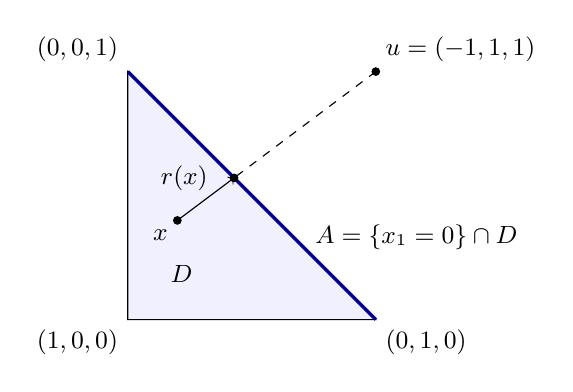
\begin{tikzpicture}[scale=1.05, every node/.style={font=\small}]
\coordinate (U) at (3,3);
\coordinate (Eone) at (0,0);
\coordinate (Etwo) at (3,0);
\coordinate (Ethree) at (0,3);
\coordinate (X) at (.6,1.2);
\coordinate (R) at (1.285714,1.714286);
\fill[blue!6] (Eone)--(Etwo)--(Ethree)--cycle;
\draw (Eone)--(Etwo)--(Ethree)--cycle;
\draw[very thick,blue!60!black] (Etwo)--(Ethree);
\draw[dashed] (U)--(R);
\draw[->] (X)--(R);
\fill (U) circle (1.5pt) node[above right] {\(u=(-1,1,1)\)};
\fill (X) circle (1.5pt) node[below left] {\(x\)};
\fill (R) circle (1.5pt) node[left=6pt] {\(r(x)\)};
\node[below left] at (Eone) {\((1,0,0)\)};
\node[below right] at (Etwo) {\((0,1,0)\)};
\node[above left] at (Ethree) {\((0,0,1)\)};
\node at (.65,.55) {\(D\)};
\node[right] at (2.15,1.0) {\(A=\{x_1=0\}\cap D\)};
\end{tikzpicture}
\caption{The affine plane \(x_1+x_2+x_3=1\), drawn using
\((x_2,x_3)\) as coordinates. The triangle is \(D\), and its thick
edge is the deleted union \(A\). The point \(r(x)\) is the first
point of \(D\) on the ray from \(u\) through \(x\); the homotopy
moves \(x\) along the indicated segment to that edge.}
\label{fig:deleted-face}
\end{figure}

\begin{remark}[The visible-face alternative]\label{rem:visible-faces}
Stanley discusses the visible-boundary case in
\cite[discussion preceding and proof of Proposition~8.3]{Stanley1974Reciprocity}.
Here it also gives a short geometric proof covering degenerate polytopes.
With \(D\ne\varnothing\) and \(I\ne\varnothing\), the preceding
coordinate calculation identifies \(A\) as exactly the first entry
points of rays from \(u\) into \(D\). Indeed, for \(a\in A\),
a coordinate with \(a_i=0\), \(i\in I\), stays negative on the
segment from \(u\) preceding \(a\).
By strict separation, choose a linear functional \(f\) and \(c>0\) with
\(f(x-u)>c\) on \(D\), and project centrally onto
\(H=\{z:f(z-u)=c\}\):
\[
\pi(x)=u+\frac{c(x-u)}{f(x-u)}.
\]
There is one first entry point on each ray meeting \(D\), so
\(\pi|_A\) is a continuous bijection onto \(\pi(D)\), hence a
homeomorphism by compactness. The image is convex: it is the section
by \(H\) of the convex cone with vertex \(u\) generated by \(D\).
Thus \(A\) is homeomorphic to a nonempty compact convex set and
\(\chi(A)=1\), also for lower-dimensional and singleton polytopes.
Both proofs concern \(\chi(D)-\chi(A)\); one must not replace
that difference by the ordinary Euler characteristic of the nonclosed
set \(D\setminus A\).
\end{remark}

\subsection{Localization and the anticanonical character}
\label{subsec:localization}

We now identify the lattice domains in the fixed-point formula. The two
lemmas above will determine their constant terms component by component.

\begin{proof}[Proof of Theorem~\ref{thm:index}]
Write \(\Lambda=\operatorname{Hom}(T,S^1)\) for the character lattice
and \(t^\lambda\) for the value at \(t\in T\) of a character
\(\lambda\in\Lambda\). The invariant index is the coefficient of
\(t^0\) in the alternating character.

The Dolbeault complex is an equivariant elliptic complex on any compact
complex manifold; a K\"ahler metric is not needed for its index.
For elements generating dense cyclic subgroups of \(T\), the fixed
locus is \(F^T\). If \(F^T\) is empty, the fixed-point theorem makes
the entire alternating character zero on these elements. Such elements
are dense in \(T\), and the character of a finite-dimensional virtual
representation is continuous, hence identically zero. In this case
\(I_T(m)=0\) for all \(m\), including zero, and we take \(P=0\).
Otherwise apply the equivariant Dolbeault fixed-point formula on the
dense set of these elements. Clearing its finitely many denominators
gives an identity of rational characters.
Its compact-group form, including fixed components, follows from
\cite[Theorem~2.12 and \S3]{AtiyahSegal1968} and
\cite[Theorems~3.9 and 4.3]{AtiyahSinger1968}.
For a component \(Z\) of \(F^T\), write \(\nu_i\ne0\) for the normal
tangent characters, repeated with their ranks, and \(x_i\) for the
corresponding formal Chern roots. The natural anticanonical fiber
weight is
\[
w=\sum_i\nu_i.
\]
Writing \(L=K_F^{-1}\), the contribution to the alternating character
is
\begin{equation}\label{eq:localization}
\int_Z \td(Z)\,e^{m c_1(L|_Z)}\,t^{mw}
\prod_i\frac1{1-t^{-\nu_i}e^{-x_i}}.
\end{equation}
The action on sections uses the inverse action on arguments, accounting
for the conormal characters in the denominator.
Choose an integral one-parameter direction pairing nontrivially with
every normal character at every fixed component.
For a component \(Z\), let \(I\) be the indices with positive pairing.
Put \(\alpha_i=\nu_i\) on \(I\), and \(\alpha_i=-\nu_i\) otherwise.
All \(\alpha_i\) pair positively with the chosen direction.
The pairings are positive integers, hence at least one.
Expand the denominators toward exponents with positive pairing:
\[
\frac1{1-t^{-\nu_i}e^{-x_i}}
=
\begin{cases}
-\displaystyle\sum_{b_i>0}t^{b_i\alpha_i}e^{b_ix_i},
&i\in I,\\[6pt]
\displaystyle\sum_{b_i\ge0}t^{b_i\alpha_i}e^{-b_ix_i},
&i\notin I.
\end{cases}
\]
These expansions respect the identity of rational characters in a
completion in which there are only finitely many terms below each
pairing bound. In particular, each trivial-character coefficient is
a finite sum.

The coefficient of the trivial character in \eqref{eq:localization}
is therefore a polynomially weighted lattice count satisfying
\[
\sum_i\alpha_i b_i=-mw,\qquad
b_i>0\ (i\in I),\quad b_i\ge0\ (i\notin I).
\]
Before integration, the polynomial weight in the truncated root space is
\begin{equation}\label{eq:lattice-weight}
W(b,m)=(-1)^{|I|}\left[
\td(Z)\exp\!\left(m c_1(L|_Z)
 +\sum_{i\in I}b_i x_i-\sum_{i\notin I}b_i x_i\right)
\right]_{\le\dim Z}.
\end{equation}
The bracket retains complex cohomological degrees at most \(\dim Z\),
so only finitely many terms contribute and \(W\) is polynomial in
\(b,m\). The sign is part of this weight.
All root expressions are interpreted by the splitting principle in
truncated cohomological degrees. Operations are first performed
coefficientwise with formal roots. Individual root monomials or
individual face terms need not define cohomology classes. Permuting
roots within an equal-character normal bundle, together with the
corresponding lattice coordinates, preserves the entire lattice domain
and its total weighted sum. Thus the complete sum is symmetric at
every positive divisible exponent. Its polynomial continuation is
symmetric coefficient by coefficient, by uniqueness of a polynomial
on an infinite progression. Only after taking this complete sum do we
interpret the symmetric polynomials as characteristic classes and
integrate on \(Z\).

For positive \(m\), the domain is the dilation by \(m\) of the rational
compact polytope
\begin{equation}\label{eq:D}
D=\left\{b_i\ge0:\ \sum_i\alpha_i b_i=-w\right\},
\end{equation}
with the union \(A\) of its faces \(b_i=0\), \(i\in I\), removed.

If \(I=\varnothing\), then \(-w=\sum_i\alpha_i\), so \(D\ne\varnothing\).
Lemma~\ref{lem:ehrhart} gives the polynomial continuation, whose
constant term is the weight at \((b,m)=(0,0)\).
If \(I\ne\varnothing\) and \(D\) is empty, the contribution is zero.
Otherwise the vector with coordinates \(-1\) on \(I\) and \(1\)
elsewhere belongs to the affine equation space in \eqref{eq:D},
since the linearization is anticanonical.
Lemma~\ref{lem:faces} gives \(\chi(A)=\chi(D)=1\).
By inclusion--exclusion and Lemma~\ref{lem:ehrhart}, the polynomial
constant term of the count on \(D\setminus A\) is
\[
\bigl(\chi(D)-\chi(A)\bigr)W(0,0)=0.
\]

These constants are exactly the actual trivial-character contributions
at \(m=0\). Indeed, positivity of the pairing forces every \(b_i=0\)
when \(\sum\alpha_i b_i=0\); this is permitted precisely when
\(I=\varnothing\). Summing over fixed components and taking a common
divisibility integer proves both polynomiality and \(P(0)=I_T(0)\).
An empty normal list gives the one-point lattice domain in \(\R^0\),
with no deleted faces; its contribution is the ordinary index integral
on that fixed component. This also handles a trivial torus. The empty
fixed set was handled before localization.
Finally, the polynomial has rational coefficients because its values at
all positive points of an integral progression are integers.
\end{proof}

\subsection{Invariant twisted forms}

The index theorem is independent of positivity. For its geometric
application we now assume K\"ahlerness and introduce the analytic map
that turns cohomology into holomorphic forms.

\begin{theorem}[Hard Lefschetz with semipositive coefficients]
\label{thm:lef}
Let \(F\) be compact Kähler of dimension \(n\), with Kähler form
\(\omega\), and let \(A\) have a smooth semipositive Hermitian metric.
For every \(0\le q\le n\), wedge multiplication by \(\omega^q\) induces a
surjection
\[
H^0(F,\Omega_F^{n-q}\otimes A)
\longrightarrow H^q(F,K_F\otimes A).
\]
\end{theorem}

This is the smooth-metric case of
\cite[Theorem~0.1]{DPS2001}; its multiplier ideal is trivial.
The smooth-coefficient Lefschetz theorem of Mourougane
\cite[Theorem~2.6]{Mourougane1999} and the earlier nef-coefficient
cohomology work of Takegoshi \cite[Theorem~1]{Takegoshi1997} are
antecedents of this statement. We use the formulation in \cite{DPS2001}.
If a compact group preserves the data, the map is equivariant. Averaging
over the group then preserves surjectivity on invariant subspaces.

\begin{corollary}\label{cor:invariantforms}
Let \(F\) be compact Kähler with smoothly semipositive
\(L_F=-K_F\), and let a compact torus \(T\) act holomorphically,
with the natural linearization on \(L_F\). If
\[
\sum_q(-1)^q\dim H^q(F,\OO_F)^T\ne0,
\]
then for some fixed \(p\ge0\) and arbitrarily large positive integers
\(m\),
\[
H^0(F,\Omega_F^p\otimes L_F^{m+1})^T\ne0.
\]
\end{corollary}

\begin{proof}
By Theorem~\ref{thm:index}, \(I_T(m)\ne0\) for all but finitely many
positive integers in a divisible progression. Some fixed \(q\)
therefore has \(H^q(F,L_F^m)^T\ne0\) for unbounded \(m\).
Average a Kähler form over \(T\), and apply
Theorem~\ref{thm:lef} with \(A=L_F^{m+1}\). Its target is
\[
H^q(F,K_F\otimes L_F^{m+1})=H^q(F,L_F^m).
\]
The wedge map is equivariant, and compact averaging gives an invariant
preimage of each invariant target class. Take \(p=\dim F-q\).
Indeed the map is \(u\mapsto[\omega^q\wedge u]\); it depends on the
averaged K\"ahler form and the natural linearization, not on the
coefficient metric used to establish surjectivity. Averaging a chosen
preimage over Haar probability measure therefore leaves its invariant
target unchanged.
\end{proof}
